\documentclass{standalone}
\usepackage{tikz}
\usetikzlibrary{patterns, positioning}

\begin{document}
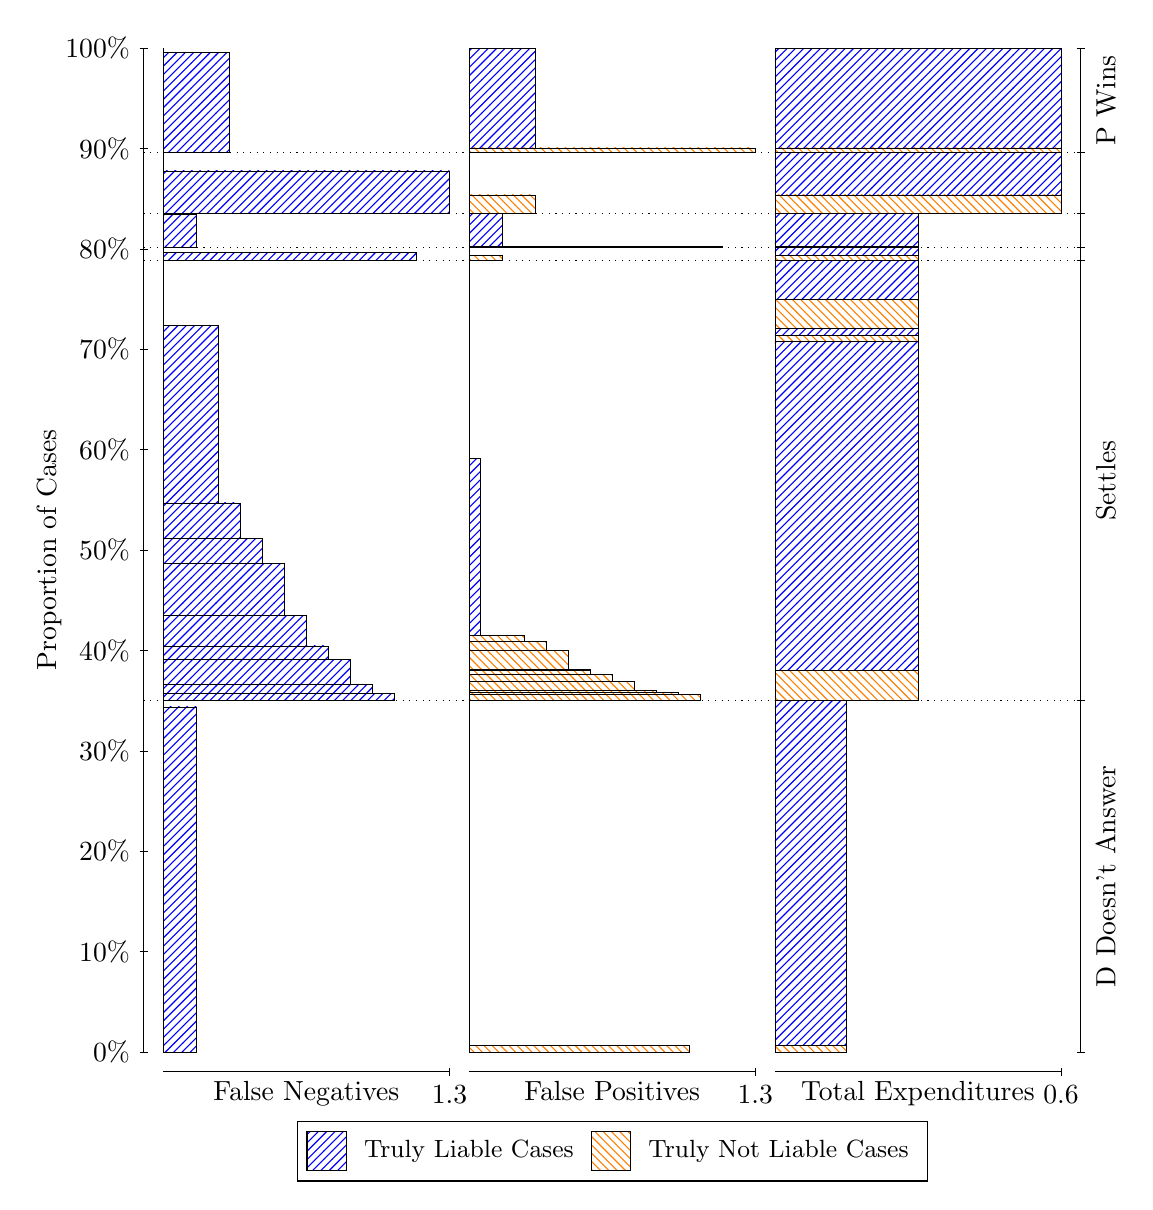
\begin{tikzpicture}
\draw[black, very thin] (1.5,1.75) -- (1.5,14.5);
\node[rotate=90, anchor=center] at (0.3, 8.125) {Proportion of Cases};
\draw[black, very thin] (1.45,1.75) -- (1.55,1.75);
\node[anchor=east] at (1.45, 1.75) {0\%};
\draw[black, very thin] (1.45,3.025) -- (1.55,3.025);
\node[anchor=east] at (1.45, 3.025) {10\%};
\draw[black, very thin] (1.45,4.3) -- (1.55,4.3);
\node[anchor=east] at (1.45, 4.3) {20\%};
\draw[black, very thin] (1.45,5.575) -- (1.55,5.575);
\node[anchor=east] at (1.45, 5.575) {30\%};
\draw[black, very thin] (1.45,6.85) -- (1.55,6.85);
\node[anchor=east] at (1.45, 6.85) {40\%};
\draw[black, very thin] (1.45,8.125) -- (1.55,8.125);
\node[anchor=east] at (1.45, 8.125) {50\%};
\draw[black, very thin] (1.45,9.4) -- (1.55,9.4);
\node[anchor=east] at (1.45, 9.4) {60\%};
\draw[black, very thin] (1.45,10.675) -- (1.55,10.675);
\node[anchor=east] at (1.45, 10.675) {70\%};
\draw[black, very thin] (1.45,11.95) -- (1.55,11.95);
\node[anchor=east] at (1.45, 11.95) {80\%};
\draw[black, very thin] (1.45,13.225) -- (1.55,13.225);
\node[anchor=east] at (1.45, 13.225) {90\%};
\draw[black, very thin] (1.45,14.5) -- (1.55,14.5);
\node[anchor=east] at (1.45, 14.5) {100\%};

\draw[black, very thin] (13.4,1.75) -- (13.4,14.5);
\draw[black, very thin] (13.35,1.75) -- (13.45,1.75);
\node[anchor=west] at (13.35, 1.75) {};
\draw[black, very thin] (13.35,6.2106) -- (13.45,6.2106);
\node[anchor=west] at (13.35, 6.2106) {};
\draw[black, very thin] (13.35,11.8) -- (13.45,11.8);
\node[anchor=west] at (13.35, 11.8) {};
\draw[black, very thin] (13.35,11.97) -- (13.45,11.97);
\node[anchor=west] at (13.35, 11.97) {};
\draw[black, very thin] (13.35,12.403) -- (13.45,12.403);
\node[anchor=west] at (13.35, 12.403) {};
\draw[black, very thin] (13.35,13.172) -- (13.45,13.172);
\node[anchor=west] at (13.35, 13.172) {};
\draw[black, very thin] (13.35,14.5) -- (13.45,14.5);
\node[anchor=west] at (13.35, 14.5) {};

\draw[black, very thin, pattern color=blue, pattern=north east lines] (1.75,1.75) rectangle (2.1692,6.1313);
\draw[black, very thin, pattern color=orange, pattern=north west lines] (1.75,6.1313) rectangle (1.75,6.2106);
\draw[black, very thin, pattern color=blue, pattern=north east lines] (1.75,6.2106) rectangle (4.6846,6.3012);
\draw[black, very thin, pattern color=blue, pattern=north east lines] (1.75,6.3012) rectangle (4.4051,6.418);
\draw[black, very thin, pattern color=blue, pattern=north east lines] (1.75,6.418) rectangle (4.1256,6.7393);
\draw[black, very thin, pattern color=blue, pattern=north east lines] (1.75,6.7393) rectangle (3.8462,6.9064);
\draw[black, very thin, pattern color=blue, pattern=north east lines] (1.75,6.9064) rectangle (3.5667,7.2954);
\draw[black, very thin, pattern color=blue, pattern=north east lines] (1.75,7.2954) rectangle (3.2872,7.9508);
\draw[black, very thin, pattern color=blue, pattern=north east lines] (1.75,7.9508) rectangle (3.0077,8.271);
\draw[black, very thin, pattern color=blue, pattern=north east lines] (1.75,8.271) rectangle (2.7282,8.7247);
\draw[black, very thin, pattern color=blue, pattern=north east lines] (1.75,8.7247) rectangle (2.4487,10.974);
\draw[black, very thin, pattern color=orange, pattern=north west lines] (1.75,10.974) rectangle (1.75,11.8);
\draw[black, very thin, pattern color=blue, pattern=north east lines] (1.75,11.8) rectangle (4.9641,11.901);
\draw[black, very thin, pattern color=orange, pattern=north west lines] (1.75,11.901) rectangle (1.75,11.97);
\draw[black, very thin, pattern color=blue, pattern=north east lines] (1.75,11.97) rectangle (2.1692,12.393);
\draw[black, very thin, pattern color=orange, pattern=north west lines] (1.75,12.393) rectangle (1.75,12.403);
\draw[black, very thin, pattern color=blue, pattern=north east lines] (1.75,12.403) rectangle (5.3833,12.94);
\draw[black, very thin, pattern color=orange, pattern=north west lines] (1.75,12.94) rectangle (1.75,13.172);
\draw[black, very thin, pattern color=blue, pattern=north east lines] (1.75,13.172) rectangle (2.5885,14.441);
\draw[black, very thin, pattern color=orange, pattern=north west lines] (1.75,14.441) rectangle (1.75,14.5);
\draw[black, very thin, pattern color=orange, pattern=north west lines] (5.6333,1.75) rectangle (8.4282,1.8293);
\draw[black, very thin, pattern color=blue, pattern=north east lines] (5.6333,1.8293) rectangle (5.6333,6.2106);
\draw[black, very thin, pattern color=orange, pattern=north west lines] (5.6333,6.2106) rectangle (8.5679,6.2899);
\draw[black, very thin, pattern color=orange, pattern=north west lines] (5.6333,6.2899) rectangle (8.2885,6.313);
\draw[black, very thin, pattern color=orange, pattern=north west lines] (5.6333,6.313) rectangle (8.009,6.3396);
\draw[black, very thin, pattern color=orange, pattern=north west lines] (5.6333,6.3396) rectangle (7.7295,6.4526);
\draw[black, very thin, pattern color=orange, pattern=north west lines] (5.6333,6.4526) rectangle (7.45,6.5472);
\draw[black, very thin, pattern color=orange, pattern=north west lines] (5.6333,6.5472) rectangle (7.1705,6.5936);
\draw[black, very thin, pattern color=orange, pattern=north west lines] (5.6333,6.5936) rectangle (7.1705,6.613);
\draw[black, very thin, pattern color=orange, pattern=north west lines] (5.6333,6.613) rectangle (6.891,6.8495);
\draw[black, very thin, pattern color=orange, pattern=north west lines] (5.6333,6.8495) rectangle (6.6115,6.9604);
\draw[black, very thin, pattern color=orange, pattern=north west lines] (5.6333,6.9604) rectangle (6.3321,7.0367);
\draw[black, very thin, pattern color=blue, pattern=north east lines] (5.6333,7.0367) rectangle (5.7731,9.2861);
\draw[black, very thin, pattern color=blue, pattern=north east lines] (5.6333,9.2861) rectangle (5.6333,11.8);
\draw[black, very thin, pattern color=orange, pattern=north west lines] (5.6333,11.8) rectangle (6.0526,11.869);
\draw[black, very thin, pattern color=blue, pattern=north east lines] (5.6333,11.869) rectangle (5.6333,11.97);
\draw[black, very thin, pattern color=orange, pattern=north west lines] (5.6333,11.97) rectangle (8.8474,11.979);
\draw[black, very thin, pattern color=blue, pattern=north east lines] (5.6333,11.979) rectangle (6.0526,12.403);
\draw[black, very thin, pattern color=orange, pattern=north west lines] (5.6333,12.403) rectangle (6.4718,12.634);
\draw[black, very thin, pattern color=blue, pattern=north east lines] (5.6333,12.634) rectangle (5.6333,13.172);
\draw[black, very thin, pattern color=orange, pattern=north west lines] (5.6333,13.172) rectangle (9.2667,13.231);
\draw[black, very thin, pattern color=blue, pattern=north east lines] (5.6333,13.231) rectangle (6.4718,14.5);
\draw[black, very thin, pattern color=orange, pattern=north west lines] (9.5167,1.75) rectangle (10.425,1.8293);
\draw[black, very thin, pattern color=blue, pattern=north east lines] (9.5167,1.8293) rectangle (10.425,6.2106);
\draw[black, very thin, pattern color=orange, pattern=north west lines] (9.5167,6.2106) rectangle (11.333,6.5936);
\draw[black, very thin, pattern color=blue, pattern=north east lines] (9.5167,6.5936) rectangle (11.333,10.773);
\draw[black, very thin, pattern color=orange, pattern=north west lines] (9.5167,10.773) rectangle (11.333,10.849);
\draw[black, very thin, pattern color=blue, pattern=north east lines] (9.5167,10.849) rectangle (11.333,10.94);
\draw[black, very thin, pattern color=orange, pattern=north west lines] (9.5167,10.94) rectangle (11.333,11.307);
\draw[black, very thin, pattern color=blue, pattern=north east lines] (9.5167,11.307) rectangle (11.333,11.8);
\draw[black, very thin, pattern color=orange, pattern=north west lines] (9.5167,11.8) rectangle (11.333,11.869);
\draw[black, very thin, pattern color=blue, pattern=north east lines] (9.5167,11.869) rectangle (11.333,11.97);
\draw[black, very thin, pattern color=orange, pattern=north west lines] (9.5167,11.97) rectangle (11.333,11.979);
\draw[black, very thin, pattern color=blue, pattern=north east lines] (9.5167,11.979) rectangle (11.333,12.403);
\draw[black, very thin, pattern color=orange, pattern=north west lines] (9.5167,12.403) rectangle (13.15,12.634);
\draw[black, very thin, pattern color=blue, pattern=north east lines] (9.5167,12.634) rectangle (13.15,13.172);
\draw[black, very thin, pattern color=orange, pattern=north west lines] (9.5167,13.172) rectangle (13.15,13.231);
\draw[black, very thin, pattern color=blue, pattern=north east lines] (9.5167,13.231) rectangle (13.15,14.5);
\draw[black, dotted] (1.5,6.2106) -- (13.4,6.2106);
\draw[black, dotted] (1.5,11.8) -- (13.4,11.8);
\draw[black, dotted] (1.5,11.97) -- (13.4,11.97);
\draw[black, dotted] (1.5,12.403) -- (13.4,12.403);
\draw[black, dotted] (1.5,13.172) -- (13.4,13.172);
\draw[black, very thin] (1.75,1.5) -- (5.3833,1.5);
\node[anchor=north] at (3.5667, 1.5) {False Negatives};
\draw[black, very thin] (5.3833,1.45) -- (5.3833,1.55);
\node[anchor=north] at (5.3833, 1.45) {1.3};

\draw[black, very thin] (5.6333,1.5) -- (9.2667,1.5);
\node[anchor=north] at (7.45, 1.5) {False Positives};
\draw[black, very thin] (9.2667,1.45) -- (9.2667,1.55);
\node[anchor=north] at (9.2667, 1.45) {1.3};

\draw[black, very thin] (9.5167,1.5) -- (13.15,1.5);
\node[anchor=north] at (11.333, 1.5) {Total Expenditures};
\draw[black, very thin] (13.15,1.45) -- (13.15,1.55);
\node[anchor=north] at (13.15, 1.45) {0.6};

\node[black, centered, rotate=90] at (13.72, 3.9803) {D Doesn't Answer};
\node[black, centered, rotate=90] at (13.72, 9.0054) {Settles};



\node[black, centered, rotate=90] at (13.72, 13.836) {P Wins};

\draw (7.449999999999999,1.5) node[draw=none] (baseCoordinate) {};
\begin{scope}[align=center]
        \matrix[scale=0.5, draw=black, below=0.5cm of baseCoordinate, nodes={draw}, column sep=0.1cm]{
            \node[rectangle, draw, minimum width=0.5cm, minimum height=0.5cm, pattern=north east lines, pattern color=blue] {}; &
            \node[draw=none, font=\small] (B) {Truly Liable Cases}; &
            \node[rectangle, draw, minimum width=0.5cm, minimum height=0.5cm, pattern=north west lines, pattern color=orange] {}; &
            \node[draw=none, font=\small] (B) {Truly Not Liable Cases}; \\
            };
\end{scope}

\end{tikzpicture}
\end{document}